\subsection{Kubernetes Admission Controllers}

An \textit{admission controller} is a piece of code that intercepts requests to
the Kubernetes API server prior to the persistence of the object but after the
request is authenticated and authorized. Admission controllers may be
\textit{validating}, \textit{mutating}, or both. Mutating controllers may modify
related objects to the requests they admit; validating controllers may not.

The admission control process proceeds in two phases. In the first phase, it
runs the mutating admission controllers. In the second phase, it runs the
validating admission controllers. If any controller in either phase rejects the
request, the entire request is rejected immediately and an error is returned to
the end-user.

Various admission controllers come compiled into the \co{kube-apiserver} binary,
and out of them, there are two controllers of particular interest, the
\co{MutatingAdmissionWebhook} and \co{ValidatingAdmissionWebhook}:
\begin{itemize}
      \tightlist
      \item \co{MutatingAdmissionWebhook}: This admission controller calls any
            mutating webhooks which match the request. Matching webhooks are called
            serially; each one may modify the object if desired.

      \item \co{ValidatingAdmissionWebhook}: This admission controller calls any
            validating webhooks which match the request. Matching webhooks are
            called in parallel; if any of them rejects the request, the request
            fails.
\end{itemize}

The admission controller phases are shown in Figure
~\ref{figure:admission-controller}.
\begin{figure}[ht]
      \centering
      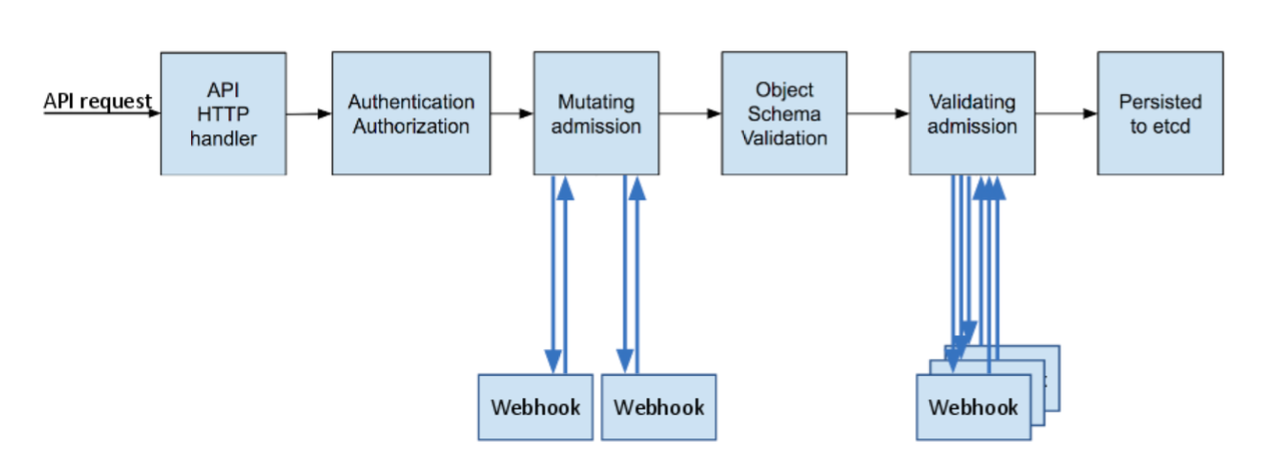
\includegraphics[width=\textwidth]{resources/admission-controller-phases.png}
      \caption{Admission controller phases}
      \label{figure:admission-controller}
\end{figure}

\section{Kubernetes Admission Webhooks}

Admission webhooks are HTTP callbacks that receive admission requests and do
something with them. Two types of admission webhooks can be defined:
\textit{validating admission} webhook and \textit{mutating admission} webhook.

Mutating admission webhooks are invoked first, and can modify objects sent to
the API server to enforce custom defaults. After all object modifications are
complete, and after the incoming object is validated by the API server,
validating admission webhooks are invoked and can reject requests to enforce
custom policies.The admin of the cluster can dynamically configure what
resources are subject to what admission webhooks via
\co{ValidatingWebhookConfiguration} or \co{MutatingWebhookConfiguration} API
objects.

\paragraph*{\co{MutatingWebhookConfiguration} Object}

Each \texttt{MutatingWebhookConfiguration} contains a list of webhooks,
specified at \co{webhooks} field. Each of the webhooks defined, may specify the
following fields:
\begin{itemize}
      \tightlist
      \item \texttt{rules}: A list of rules used to determine if a request to
            the API server should be sent to the webhook. Each rule specifies
            one or more operations, apiGroups, apiVersions, and resources, and a
            resource scope.
      \item  \texttt{failurePolicy}: Defines how unrecognized errors and timeout
            errors from the admission webhook are handled. Allowed values are
            \texttt{Ignore} or \texttt{Fail}.
      \item \texttt{namespaceSelector}:  Defines whether to run the webhook on a
            request for a namespaced resource (or a \texttt{Namespace} object) based
            on whether the namespace labels match the selector. If the object is a
            cluster scoped resource other than a Namespace, \texttt{namespaceSelector}
            has no effect.
\end{itemize}